  
 
  
  
\begin{frame}\frametitle{Factors flow graph} 
  
  
\begin{center} 
  
  
\begin{figure} 
  
  
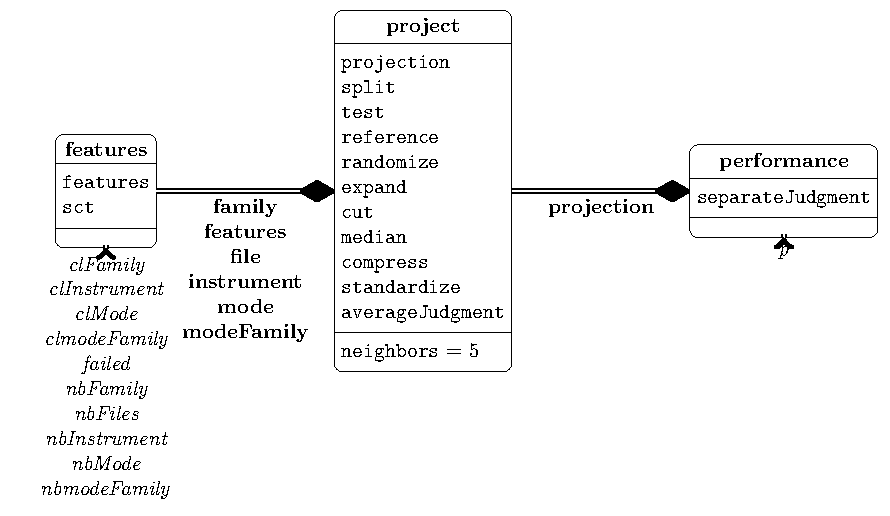
\includegraphics[width=\textwidth,height=0.8\textheight,keepaspectratio]{../figures/factors.pdf} 
  
  
\label{factorFlowGraph} 
  
  
\end{figure} 
  
  
\end{center} 
  
  
\end{frame} 
  
\begin{frame}\frametitle{sct: 1000, split: none, reference: judgments, randomize: 0, expand: 0, cut: 1, median: 1, compress: 1, standardize: 1} 
  
\begin{table} 
\begin{center} 
\ 
 \setlength{\tabcolsep}{.16667em} 
\begin{tabular}{llllc} 
features & projection & averageJudgment & separateJudgment & p (\%) \\ 
\hline 
mfcc & lmnn & 0 & 0 &  86.31 $\pm$5.91 \\ 
mfcc & lmnn & 0 & 1 &  86.18 $\pm$6.05 \\ 
mfcc & lmnn & 1 & 0 &  86.22 $\pm$5.92 \\ 
mfcc & none & 1 &  &  85.07 $\pm$6.19 \\ 
mfcc & lda & 1 &  &  81.50 $\pm$7.65 \\ 
scat & lmnn & 0 & 0 &  93.31 $\pm$3.92 \\ 
scat & lmnn & 0 & 1 & \textbf{\textcolor{red}{ 98.09 $\pm$1.28}} \\ 
scat & lmnn & 1 & 0 &  94.80 $\pm$3.26 \\ 
scat & none & 1 &  &  87.01 $\pm$5.81 \\ 
scat & lda & 1 &  & 80.95 $\pm$10.37 \\ 
\end{tabular} 
\end{center} 
\label{sc1000SpnoRejuRa0Ex0Cu1Me1Co1St1} 
\end{table} 
 
\end{frame}  
  
\begin{frame}\frametitle{\small split: none, reference: judgments, randomize: 0, expand: 0, cut: 1, median: 1, compress: 1, standardize: 1} 
\begin{center} 
\begin{figure} 
\centering 
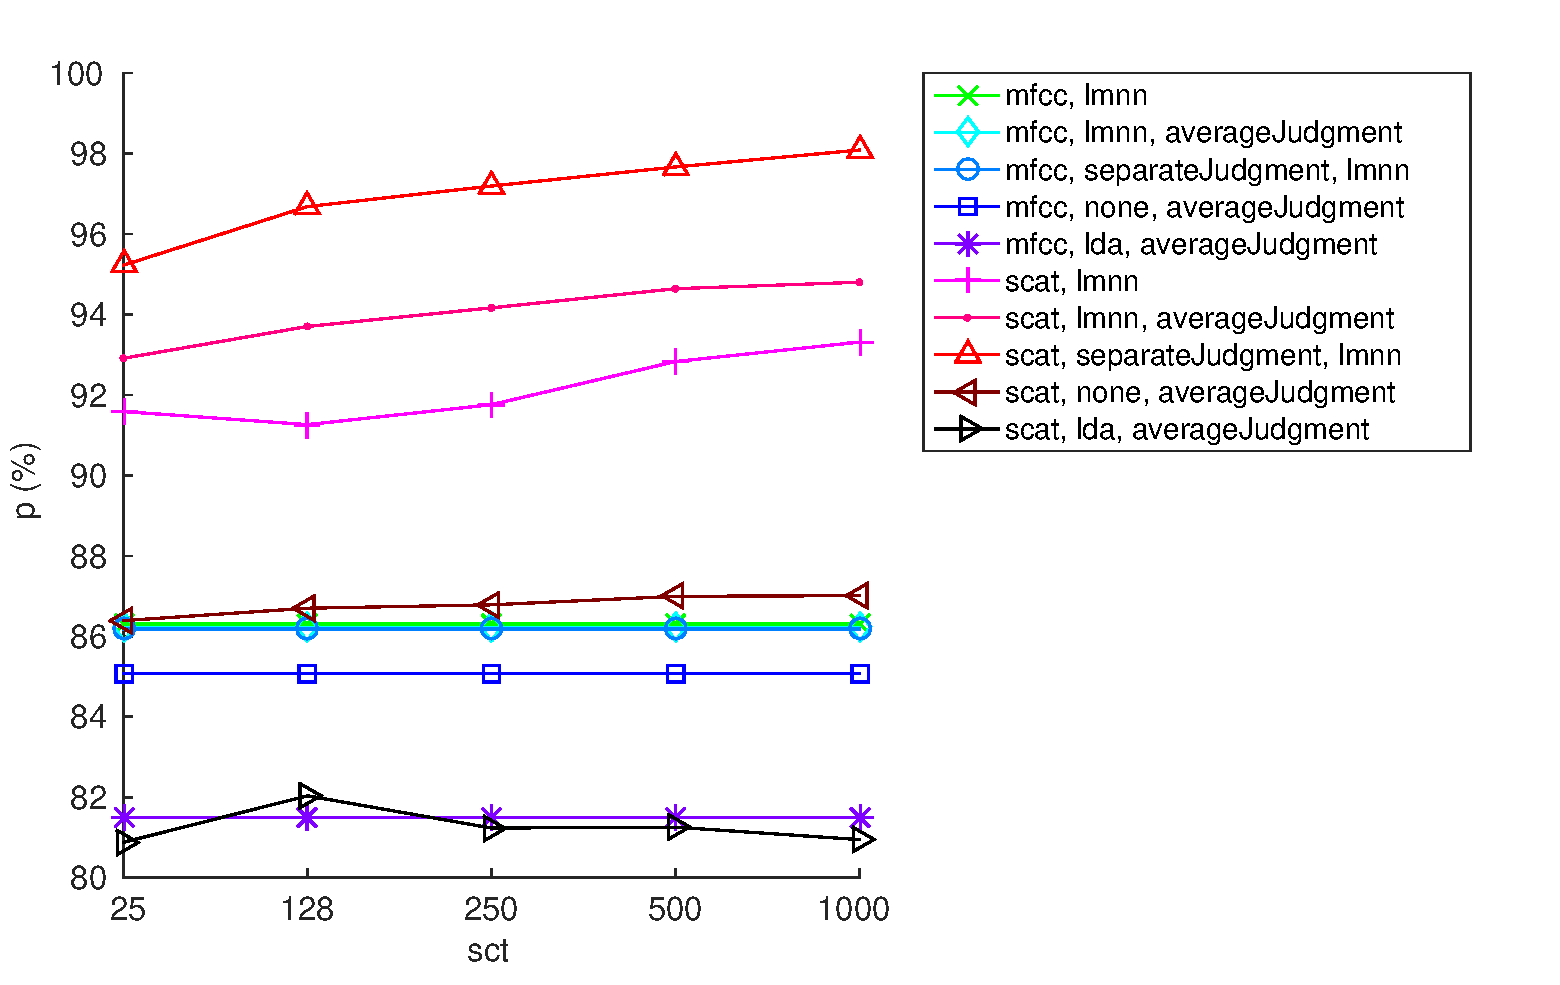
\includegraphics[width=\textwidth,height=0.8\textheight,keepaspectratio]{./figures/Fig160.pdf} 
\label{spnoRejuRa0Ex0Cu1Me1Co1St1} 
\end{figure} 
\end{center} 
  
  
\end{frame}  
